
%%%%%%%%%%%%%%%%%%%%%%%%%%%%%%%%%%%%%%%%%%%%%%%%%%%%%%%%%%%%%%
\subsection{Metric Properties of the Patch Manifold}

This paper describes the manifold structure of $\Mm$ for various image ensembles that model some typical cases of natural signals, images and textures. In order to give qualitative statements about this structure and to explore it numerically, we perform geodesic computations over this manifold. It is important to note that these geodesic computations are not actually used to solve inverse problems as explained in section \ref{sec-inverse-pbm}. They are however useful to visualize and gain further understanding about the geometry of patches manifolds.

The local metric on $\Mm$ is defined through the Euclidean embedding of the manifold $\Mm$ in $\Ldeux([-\tau/2,\tau/2]^d)$. The parameterization $\phi$ maps the metric of $\Om$ onto this manifold metric through the first fundamental form
\begin{equation*}
	\text{I}_{\Mm}(\xi) \eqdef 
	\pa{ \bdotp{ \pd{\phi(\xi)}{\xi_i} }{ \pd{\phi(\xi)}{\xi_j} } }_{i,j} \in \RR^{m \times m},
\end{equation*}
where $\dotp{\cdot}{\cdot}$ is the Euclidean inner product of $\Ldeux([-\tau/2,\tau/2]^d)$.

The length of a piecewise smooth curve $t \in [0,1] \mapsto \ga(t) \in \Mm$ on the manifold is 
\begin{equation*}
	L(\ga) \eqdef \int_0^1 \norm{\ga'(t)} \d t
\end{equation*}
and $\Mm$ can be turned into a metric space by considering the geodesic length
\begin{equation*}
	d_{\Mm}(p,q) \eqdef \underset{\ga \in \Pp(p,q)}{\argmin}\: L(\ga),
\end{equation*}
where $\Pp(p,q)$ is the set of path $\ga$ joining $p$ to $q$: $\ga(0)=p$ and $\ga(1)=q$.

The manifold $\Mm$ is locally flat if $\text{I}_{\Mm}(\xi) = \Id$ is the identity tensor. If in addition the parameter domain $\Om$ is convex, then the manifold is globally flat and thus isometric to the Euclidean space
\eq{
	\foralls (\xi,\xi') \in \Om^2, \qquad  d_{\Mm}(\phi(\xi),\phi(\xi')) = \norm{\xi-\xi'}. 
}

The curve (resp. surface) $c_g$ defined for a 1D signal (resp. 2D image) can be thought locally as a $d$-dimensional sub-manifold of $\Mm$. Excepted in simple cases, this mapping is however globally not injective and is often badly behaved in real applications. Complex data $g$ leads to a set $c_g$ with high curvature variations and self-intersections. A feature $p \in \Mm$ where this set intersects itself corresponds to points $x \neq y$ such that $p = p_x(g) \approx p_y(g)$. 


%%%%%%%%%%%%%%%%%%%%%%%%%%%%%%%%%%%%%%%%%%%%%%%%%%%%%%%%%%%%%%
\paragraph{Parameterization computation.}
The parameterization $\phi$ of $\Mm$ can be far from isometric or even not available analytically. In these cases, we estimate numerically such a low dimensional parameterization using manifold learning methods. We use the Isomap algorithm of Tenenbaum and De Silva \cite{tenenbaum-isomap} that produces a parameterization as isometric as possible. One could use alternative methods such as Locally Linear Embedding \cite{roweis-lle}, Laplacian eigenmaps \cite{belkin-laplacian-eigenmaps} or geometric diffusion \cite{coifman-geometric-diffusion}. We find Isomap useful since it is not biased by the variable sampling of the manifold that is unavoidable in numerical applications.

In order to estimate $\Mm$, one uses the set of discrete patches 
\eql{\label{eq-manifold-sampling}
	S = \enscond{p_{x_k}(g_\ell)}{x_k \in \zd, g_\ell\in \Th } \subset \RR^{\tau^d n}
} 
gathered at sampling locations $x_k$ and images $g_\ell$ evenly sampled on $\Theta$.

All manifold learning methods estimate the manifold $\Mm$ using a graph $\Gg$ whose vertices are $S$ and whose edges are nearest neighbors over the embedding space
\begin{equation*}
	(p \sim q) \in \Gg \quad \Longleftrightarrow \quad \norm{p-q} \leq \epsilon
\end{equation*}
where $\epsilon$ should be chosen carefully. 

The geodesic distance between two points $p,q$ can be estimated using the discrete geodesic distance over $\Gg$
\begin{equation*}
	d_{\Mm}(p,q) \approx \min_{p=p_0 \sim \ldots \sim p_k = q} \sum_{i=0}^{k-1} \norm{p_{i+1}-p_i}.
\end{equation*}
These quantities are computed using Dijkstra dynamic programming algorithm. The Isomap algorithm \cite{tenenbaum-isomap} computes a low dimensional position $\tilde p = \phi^{-1}(p)$ for every $p \in S$ by minimizing the isometric distortion
\begin{equation*}
	\pa{\tilde p_i}_{i} = 
	\underset{(q_i)_i}{\argmin} \sum_{i} \babs{ \norm{ p_i - q_i }^2 - d_{\Mm}(p_i,q_i)^2 }^2.
\end{equation*}
This non-linear problem can be minimized iteratively until one reaches a local minimum or can be replaced by an approximated quadratic energy, see \cite{tenenbaum-isomap}. In some cases, the dimensionality $m$ of the parameter space is known from the signal model $\Theta$. However, for complex sets of images, the estimation of this dimension is a complex task, see for instance \cite{camastra-dim-estimation,farahmand-manifold-adaptive}.

%%%%%%%%%%%%%%%%%%%%%%%%%%%%%%%%%%%%%%%%%%%%%%%%%%%%%%%%%%%%%%
%%%%%%%%%%%%%%%%%%%%%%%%%%%%%%%%%%%%%%%%%%%%%%%%%%%%%%%%%%%%%%
%%%%%%%%%%%%%%%%%%%%%%%%%%%%%%%%%%%%%%%%%%%%%%%%%%%%%%%%%%%%%%


\myfigure{
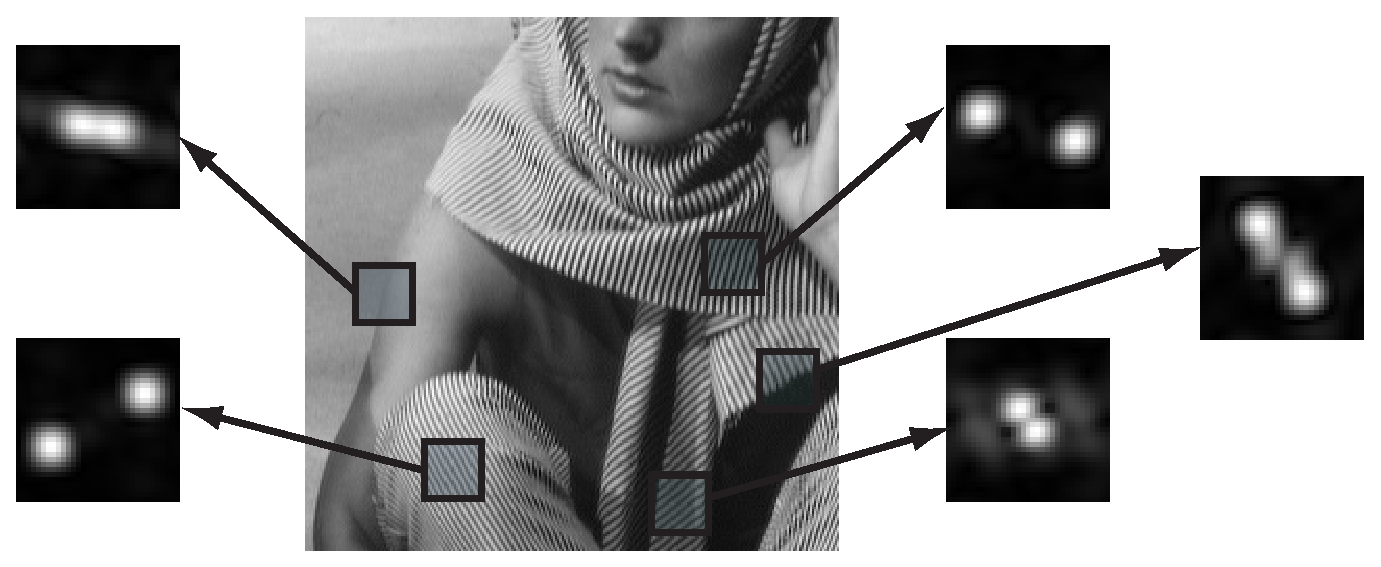
\includegraphics[width=\linewidth]{barb-patches-spectrum.eps}
}{
Examples of local Fourier expansions showing the estimation of the local phase parameters $(\rho(x),\th(x),\de(x))$. 
}{fid-local-fourier-2d}


\myfigure{
\includegraphics[width=0.32\linewidth]{locally-parallel/texture-proj-iter1.png}
\includegraphics[width=0.32\linewidth]{locally-parallel/texture-regularity-high.png}
\includegraphics[width=0.32\linewidth]{locally-parallel/texture-varying-horizontal.png}
}{
Examples of locally parallel textures with various phase properties. 
}{fid-locally-parallel-textures}

%%%%%%%%%%%%%%%%%%%%%%%%%%%%%%%%%%%%%%%%%%%%%%%%%%%%%%%%%%%%%%
%%%%%%%%%%%%%%%%%%%%%%%%%%%%%%%%%%%%%%%%%%%%%%%%%%%%%%%%%%%%%%
%%%%%%%%%%%%%%%%%%%%%%%%%%%%%%%%%%%%%%%%%%%%%%%%%%%%%%%%%%%%%%
\section{Manifold of Isolated and Periodic Patterns}
\label{sect-manifold-patterns}

%%%%%%%%%%%%%%%%%%%%%%%%%%%%%%%%%%%%%%%%%%%%%%%%%%%%%%%%%%%%%%
\subsection{Isolated patterns.}

Natural textures are often composed of similar patterns distributed over the image plane. Such a texture can be decomposed as
\begin{equation*}
	f(x) = \sum_{i=1}^k h(x-c_i)
\end{equation*}
where $h$ is the elementary pattern, which is supposed to have a compact support over $[-s/2,s/2]^2$, where $s$ should be comparable to $\tau$ in order for the patch manifold to capture the geometry of the texture. We further impose that the patterns are well separated which leads to the following texture ensemble
\begin{equation*}
	\Th = \enscond{ \sum_{i=1}^k h(x-c_i) }{ k>0 \qandq \foralls i\neq j, \norm{c_i-c_j}>s+\tau}
\end{equation*}


All the patches extracted from $f$ can thus be written as
\begin{equation*}
	p_x(f)(t) = h(t-c(x))
	\qqwhereqq c(x) = \underset{1 \leq i \leq k}{\argmin} \norm{x-c_i}.
\end{equation*}
The function $c$ is thus piecewise constant with $c(x)=c_i$ for every point $x$ in the Voronoi region 
\begin{equation*}
	V_i = \enscond{x}{\foralls j \neq i, \norm{x-c_i} \leq \norm{x-c_j}}.
\end{equation*} 
The patch manifold is thus composed of translation of the pattern $h$ and can be parameterized as
\begin{equation*}
	\Mm = \{h(\cdot-c)\}_{|c| \leq s}
	\qqandqq 
	\phi : c \mapsto h(\cdot-c)
\end{equation*}	
where $h(\cdot-c)$ is the 2D function $x \in [-\tau,\tau]^2 \mapsto f(x-c)$. The geometry of $\Mm$ depends heavily on the properties of the pattern $h$ and in particular on its regularity. When $h$ has edges, the manifold $\Mm$ is highly curved since $\nabla_c \phi = -\nabla h(\cdot - c)$ is rapidly varying when $c$ changes. Donoho and Grimes \cite{donoho-isomap} and Wakin et al. \cite{wakin-multiscale-structure} study in detail the regularity of this manifold of translations and prove that it is locally flat for a shape $h$ with 4-fold symmetries.

%%%%%%%%%%%%%%%%%%%%%%%%%%%%%%%%%%%%%%%%%%%%%%%%%%%%%%%%%%%%%%
\subsection{Periodic patterns}

To remove the condition that elementary texture patterns should be well separated and still have a simple underlying manifold, one needs to assume that the patterns are packed in a periodic way. To that end we define the vectors $V = \transp{[v_1, v_2]} \in \RR^{2\times 2}$ of a 2D lattice and suppose that the texture can be written as a periodic tiling 
\begin{equation*}
	f(x) = h( (V^{-1} x) \mod s )
\end{equation*}
where the modulo operator is taken component wise. The resulting manifold of patches is then parameterized by
\begin{equation*}
	\phi : a \in \Sun \times \Sun \mapsto P_a
	\qqwhereqq
	P_a(t) \mapsto h( (V^{-1} t) + a \mod s )
\end{equation*}
where the set of real numbers modulo $s$ is identified with the circle $\Sun$.
Natural textures often deviate from strict periodicity and more advanced processings should be used to identify a suitable irregular lattice \cite{liu-periodicity-directionality,liu-promise}. The resulting manifold of these approximately periodic textures is less trivial and cannot be parameterized by $\Sun \times \Sun$. Figure \ref{fig-manifold-periodic} shows two examples of such approximately periodic textures, together with the corresponding Euclidean and geodesic distances.

\myfigure{
\begin{tabular}{ccc}
%\figitemraise{1.5cm}{a}&
\includegraphics[width= 0.26\linewidth]{manifold/dead_leaf/dead_leaf-original.png}&
\includegraphics[width= 0.26\linewidth]{manifold/dead_leaf/dead_leaf-euclidean-dist.png}&
\includegraphics[width= 0.26\linewidth]{manifold/dead_leaf/dead_leaf-geodesic-dist.png}\\
%\figitemraise{1.5cm}{b}&
\includegraphics[width=0.26\linewidth]{manifold/reptilskin/reptilskin-original.png}&
\includegraphics[width=0.26\linewidth]{manifold/reptilskin/reptilskin-euclidean-dist.png}&
\includegraphics[width=0.26\linewidth]{manifold/reptilskin/reptilskin-geodesic-dist.png}\\[-3mm]
Image $f$ & Euclidean distance & Geodesic distance\\[2mm]
\end{tabular}
%\begin{tabular}{cc}
%\includegraphics[width=0.48\linewidth]{manifold/fabric2/fabric2-manifold-3d.png}&
%\includegraphics[width=0.48\linewidth]{manifold/reptilskin/reptilskin-manifold-3d.png}\\
%Isomap 2D reduction of \textbf{(a)} &  Isomap 2D reduction of \textbf{(b)}
%\end{tabular}
}{
Geodesic computation on manifolds of periodic patterns.
%
}{fig-manifold-periodic}



%%%%%%%%%%%%%%%%%%%%%%%%%%%%%%%%%%%%%%%%%%%%%%%%%%%%%%%%%%%%%%
\paragraph{Texture synthesis.} 
In order to perform texture synthesis, one needs to draw uniformly at random a texture $f \in \Th$. This involves finding a set of patches $p_x$ that are $k$ sparse and that overlap in a coherent manner to create a texture $f$. In order to avoid degenerate solutions such as $f=0$, one typically imposes additional constraints such as the equality of histograms between $f$ and $f_e$. This texture synthesis can thus be thought as an inverse problem, which can in turn be solved thanks to the iterative algorithm \ref{listing-iterative-projection}. The synthesized texture converged to a local stationary point of the energy \ref{eq-regularized-inversion} with $E=E_{\Mm}$.


\begin{listing}
\begin{enumerate}
	\item \textit{Initialization:} set $f$ at random.
	\item \textit{Sparse code:} for all locations $x$, compute
	\begin{equation*}
		s_x \leftarrow \Proj_{\Mm}( p_x(f) ).
	\end{equation*}
	\item \textit{Reconstruction:} compute the texture $f$ by averaging the patches
		\begin{equation*}
			f(x) = \frac{1}{n \tau^2} \sum_{|y-x| \leq \tau/2} (D s_y)(x-y).
		\end{equation*}
	\item \textit{Impose constraints:} perform the histogram equalization of $f$ with $f_e$, see \cite{peyre-sparse-textures}.
	\item \textit{Stop:} while not converged, go back to 2. 
\end{enumerate}% \vspace{-3mm}
    \caption{Sparse texture synthesis algorithm. \label{listing-texture-synthesis}}
\end{listing}


The corresponding algorithm is detailed in \ref{listing-texture-synthesis}, and is equivalent to the iterative projection algorithm of Peyr\'e \cite{peyre-sparse-textures}. This iterative algorithm can be seen as an extension of classical texture synthesis methods such as \cite{efros-nonparam-sampling,wei-texture-synthesis}. These computer graphics approaches use the highly redundant dictionary $D = \pa{p_x(f_e)}_x$ of all the patches of the exemplar $f_e$ and enforce a perfect recopy by asking a strict sparsity $k=1$. 

The texture model $\Th$ captures a compact set of parameters through the dictionary $D$. This model shares also similarity with statistical approaches to texture synthesis such as \cite{heeger-pyramid-texture,zhu-frame,portilla-parametric-model} where some transform domain randomization is performed. Whereas these approaches use a fixed wavelet transform \cite{heeger-pyramid-texture,portilla-parametric-model} or filters optimized from a fixed library \cite{zhu-frame} we learn this transform in a non-parametric fashion.
 
Figure \ref{fig-sparse-synthesis} shows examples of texture synthesis for various values of the parameters $m$ and $k$. Increasing the size of the dictionary allows for a more realistic synthesis and increasing the redundancy creates more blending between the features.

\myfigure{
\begin{tabular}{cccc}
\hspace{-3mm}\includegraphics[width=0.23\linewidth]{dictionary-learning/corral-original.png} &
\includegraphics[width=0.23\linewidth]{dictionary-learning/corral-r01s02.png}&
\includegraphics[width=0.23\linewidth]{dictionary-learning/corral-r01s08.png}&
\includegraphics[width=0.23\linewidth]{dictionary-learning/corral-r02s02.png}\\[-3mm]
% \includegraphics[width=0.3\linewidth]{dictionary-learning/corral-r02s08.png}
Original & $m/n=1, k=2$ & $m/n=1, k=8$ & $m/n=2, k=2$ \\[2mm]
\end{tabular}
}{
Examples of texture synthesis for various redundancy $m/n$ an sparsity.
%
}{fig-sparse-synthesis}





%%%%%%%%%%%%%%%%%%%%%%%%%%%%%%%%%%%%%%%%%%%%%%%%%%%%%%%%%%%%%%
\paragraph{Locally parallel texture synthesis.} 

\myfigure{
\includegraphics[width=0.32\linewidth]{locally-parallel/texture-proj-iter1.png}
\includegraphics[width=0.32\linewidth]{locally-parallel/texture-regularity-high.png}
\includegraphics[width=0.32\linewidth]{locally-parallel/texture-varying-horizontal.png}
}{
Examples of locally parallel textures with various phase properties. 
}{fid-locally-parallel-textures}

\begin{listing}
\begin{enumerate}
	\item \textit{Initialization:} set $\Phase_0 \leftarrow $ random and $k \leftarrow 0$.
	\item \textit{Compute the flow field:} normalize the gradient of the phase as follow 
		\eq{
			v_{k+1}(x) = g(x) \frac{\nabla_x \Phase_k }{ |\nabla_x \Phase_k }.
		}
	\item \textit{Compute the potential field:} $\Phase_{k+1}$ is solution of the Poisson equation 
		\eq{ 
			\Delta \Phase_{k+1} = \text{div}(v_{k+1}),
		}
		with periodic boundary conditions.
	\item \textit{Stopping criterion:} while not converged, set $k \leftarrow k+1$ and go back to 2.
	If converged, output $f(x) = \cos(\Phase_{k+1}(x))$.
\end{enumerate}% \vspace{-3mm}
    \caption{Synthesis of a locally parallel texture. \label{listing-synth-locpar}}
\end{listing}
These textures have been synthesized using the algorithm detailed in pseudo-code \ref{listing-synth-locpar}. These iterations are iterative projections on the linear constraint $\nabla \wedge v = 0$ and the manifold constraint $|v(x)|=g(x)$ starting from the initial field $v=\nabla \Phase_0$. Such iterative projections have been proven to converge locally by Lewis and Malick \cite{lewis-alternating}. 




Figure \ref{fig-manifold-natural-locpar-textures} shows the euclidean distance $\norm{p_{x_0}(f) - p_x(f)}$ and the geodesic distance $d_{\Mm}(p_{x_0}(f), p_x(f))$ from a fixed point $x_0 \in \zun^2$. Figure \ref{fig-manifold-natural-locpar-textures}, upper row, is a synthetic texture created with the iterative projection algorithm and \ref{fig-manifold-natural-locpar-textures}, bottom row, is a natural fingerprint texture. One sees that both distances are small for pixel locations $x$ where the local orientation $\th(x)$ is close to $\th(x_0)$. The geodesic distance captures the elongated structure more efficiently and is smaller along the ridges of the texture than the euclidean distance. 

% Figure \ref{fig-manifold-natural-locpar-textures-2} shows a 2D layout that tends to preserve geodesic distances. This layout is organized in a circle that represents the $\th$ parameter. The deviation from this circle is caused by the $\de$ parameter.



\myfigure{
\begin{tabular}{ccc}
\includegraphics[width=0.26\linewidth]{manifold/locparx/locparx-original.png}&
\includegraphics[width=0.26\linewidth]{manifold/locparx/locparx-euclidean-dist.png}&
\includegraphics[width=0.26\linewidth]{manifold/locparx/locparx-geodesic-dist.png}\\
\includegraphics[width=0.26\linewidth]{manifold/fingerprint/fingerprint-original.png}&
\includegraphics[width=0.26\linewidth]{manifold/fingerprint/fingerprint-euclidean-dist.png}&
\includegraphics[width=0.26\linewidth]{manifold/fingerprint/fingerprint-geodesic-dist.png}\\[-3mm]
Image $f$ & Euclidean distance & Geodesic distance\\[2mm]
\end{tabular}
}{
Geodesic computation on manifolds of locally parallel textures.
}{fig-manifold-natural-locpar-textures}




%%%%%%%%%%%%%%%%%%%%%%%%%%%%%%%%%%%%%%%%%%%%%%%%%%%%%%%%%%%%%%
\subsection{Manifold of Piecewise Constant Signals}
\label{sec-manifold-piecewise-cst}

A simple signal ensemble is composed of piecewise constant functions 
\begin{equation*}
	\Th \eqdef \enscond{ f(x) = \sum_{i=1}^k \la_i H(x-c_i) }{ 
	\begin{array}{cccc}
	0\leq k < \infty & \text{and} & \norm{f}_{\infty}\leq 1  \quad \text{and} \\
	0 \leq c_i \leq 1 & \text{and} & \forall i\neq j, \; |c_i-c_j|>\tau 
	\end{array}
	},
\end{equation*}
where $H$ is a smoothed step $H = \tilde H * h$ and $h$ is a regular kernel with compact support in $[-s/2,s/2]$ ensuring that $f$ can be sampled without aliasing. The step function is defined as $\tilde H(x)=-1$ for $x<0$ and $\tilde H(x)=1$ otherwise. From a signal processing point of view, wavelets decompositions are optimal to approximate and process this kind of signals \cite{mallat-book} since only a finite number of non-zero wavelet coefficients remains for each approximation scale. This section gives an alternate description of these signals using a manifold model.

Each patch extracted from $f$ can be written as
\begin{equation*}
	p_x(f)(t) = a(x) + b(x) H(t-c(x))
\end{equation*}
where $c(x)$ the location of the nearest  step and where $(a(x),b(x))$ are the average value and height of the step. There is an indetermination for positions $x$ such that $|x-c_i|>\tau$ for all $i$ since in this case $p_x(f)$ does not contain any step. This patch description leads to the following manifold of step discontinuities 
\begin{align}
	\label{eq-manifold-step-1d}
	&\Mm = \enscond{ P_{(a,b,c)} \in \Ldeux([-\tau/2,\tau/2]) }{(a,b,c) \in \Om}\\
	&\qwhereq P_{(a,b,c)}(t) = a + b H(t-c).
\end{align}
with
\begin{equation*}
	\Om \eqdef \enscond{ (a,b,c) \in \RR^3 }{-\tau/2 \leq c \leq \tau/2, -1 \leq a \leq 1, 0 \leq b \leq 1 }.
\end{equation*}
The natural parameterization $(a,b,c) \mapsto P_{(a,b,c)}$ of $\Mm$ is however not smooth and even not bijective when $b=0$. Figure \ref{fig-step-function-manifold} shows on an example of signal $f(x)$ the discontinuities of $a(x)$, $b(x)$ and $c(x)$. 

\myfigure{
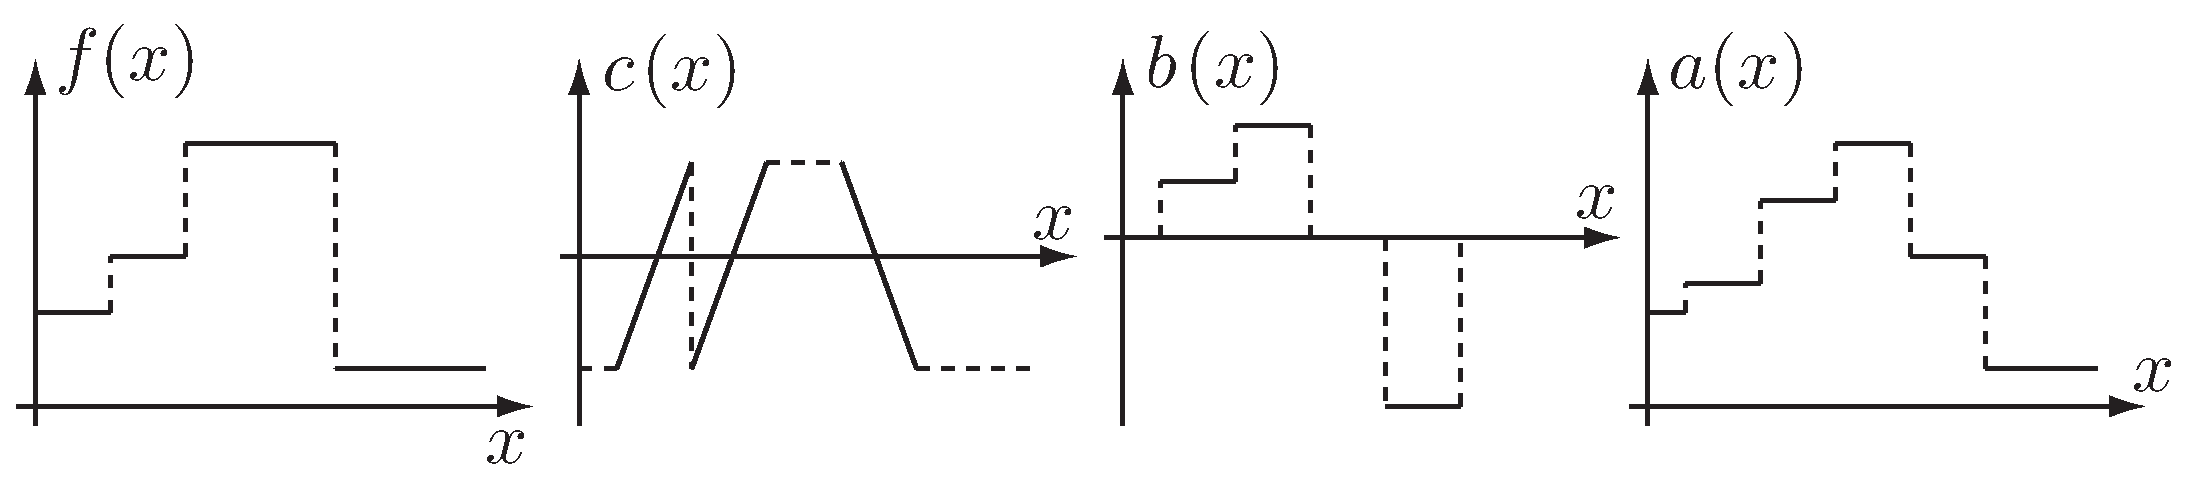
\includegraphics[width=\linewidth]{step-function-manifold.eps}
}{
A function $f$ with step discontinuities together with its parameters $(a(x),b(x),c(x))$ in the step manifold $\Mm$. 
%
}{fig-step-function-manifold}

The geometry of $\Mm$ is in fact complex and non-flat. It is estimated numerically using the isomap approach as outlined in section \ref{sect-discretization}. A large number of step patches $P_{(a,b,c)}$ are generated and Isomap is used to compute a 3D layout. It corresponds to an estimation of a parameterization $\phi^{-1}$ of $\Mm$ that is as isometric as possible. Figure \ref{fig-step-manifold-1d} shows the resulting low dimensional embedding. The black curve corresponds to an approximation of $\Cc_f$ for this parameterization of $\Mm$.


\myfigure{
\includegraphics[width=0.7\linewidth]{manifold/step1d/step1d-manifold.png}
}{
The $1D$ step manifold $\Mm$ displayed in 3D using Isomap. The black curve is the parametric representation $\tilde c_f$ of $f$ in $\Mm$.
%
}{fig-step-manifold-1d}


%%%%%%%%%%%%%%%%%%%%%%%%%%%%%%%%%%%%%%%%%%%%%%%%%%%%%%%%%%%%%%
% special affine manifold: sequential descent on the parameters

\begin{listing}
\begin{enumerate}
	\item \textit{Initialization:} set $a=1$ and $b=0$.
	\item \textit{Compute $(\th,\de)$:} perform the projection on the binary edge manifold $\Mm_0$ using a nearest neighbor search
		\eq{
			P_{(\th,\de)} = \Proj_{\Mm}( (p-b)/a ).
		}
	\item \textit{Compute $(a,b)$:} perform the least square regression, which amount to solve the following linear system in $(a,b)$
		\eq{
			\choice{
				\dotp{P_{(\th,\de)}}{P_{(\th,\de)}} a + \dotp{P_{(\th,\de)}}{1} b = \dotp{p}{P_{(\th,\de)}}, \\
				\dotp{P_{(\th,\de)}}{1} a + \dotp{1}{1} b = \dotp{p}{1}.
			}
		}
		where $1$ is the constant unit function.
	\item \textit{Stopping criterion:} while not converged, go back to 2.
\end{enumerate}% \vspace{-3mm}
    \caption{Iterative projection algorithm to compute $a P_{(\th,\de)} + b = \Proj_{\Mm}(p)$ the projection on the affine edges manifold. \label{listing-proj-affine-edges}}
\end{listing}




%%%%%%%%%%%%%%%%%%%%%%%%%%%%%%%%%%%%%%%%%%%%%%%%%%%%%%%%%%%%%%
\subsection{Manifold of Cartoon images}

On figure \ref{fig-binary-shape-functions} (b,c) one can see the parameters $\th(x)$ and $\de(x)$ of the patches $\{p_x(f)\}_x$ displayed as a 2D images. The orientation $\th(x)$ corresponds to the orientation of the boundary $\partial B$ near $x$. These functions can be expressed using the projection on  $\partial B$ and the signed distance function 
\begin{equation*}
	\pi_S(x) = \underset{y \in \partial B}{\argmin} \; \norm{x-y}
	\qqandqq 
	\Delta_S(x) = 
	\left\{
	\begin{array}{lll}
		-\norm{\pi_S(x)-x} & \text{ if } x \in B, \\
		\norm{\pi_S(x)-x} & \text{ otherwise.}
	\end{array}
	\right.
\end{equation*}
as 
\begin{equation*}
	\de(x) = \min(\max(\Delta_S(x),-\tau/2),\tau/2)
	\qqandqq
	\th(x) = \overrightarrow{N}(\pi_S(x)),
\end{equation*}
where $\overrightarrow{N}$ is the normal to the boundary of $B$. Figure \ref{fig-binary-shape-functions} (d) shows the geodesic function to some edge $p_{x_0}(f)$ located on the bottom right boundary of $B$. This distance function is computed using the Dijkstra algorithm as outlined in section \ref{sect-discretization}.


\myfigure{
\begin{tabular}{cccc}
\hspace{-5mm}\includegraphics[width=0.24\linewidth]{manifold/step2d/step2d-original.png}&
\hspace{-3mm}\includegraphics[width=0.24\linewidth]{manifold/step2d/step2d-theta.png}&
\hspace{-3mm}\includegraphics[width=0.24\linewidth]{manifold/step2d/step2d-delta.png}&
\hspace{-3mm}\includegraphics[width=0.24\linewidth]{manifold/step2d/step2d-geodesic-dist.png}\\[-3mm]
(a) Shape $1_B$ & 
\hspace{-3mm} (b) Orientation $\th(x)$ & 
\hspace{-3mm} (c) distance $\de(x)$ & 
\hspace{-5mm} (d) $d_{\Mm}(p_{x_0}(f),p_x(f))$ \\[2mm]
\end{tabular}
}{ %
Display of a smooth shape, the corresponding parameters $(\th(x),\de(x))$ of $\tilde c_f$ and the geodesic distance function. The distance ranges from 0 (blue) to its maximum value (red). %
}{fig-binary-shape-functions}

% numerics:

\myfigure{
\begin{tabular}{cccc}
\includegraphics[width=0.24\linewidth]{inpainting/piece-regular/piece-regular-iter-000.png} &
\hspace{-3mm}\includegraphics[width=0.24\linewidth]{inpainting/piece-regular/piece-regular-iter-001.png} &
\hspace{-3mm}\includegraphics[width=0.24\linewidth]{inpainting/piece-regular/piece-regular-iter-002.png} &
\hspace{-3mm}\includegraphics[width=0.24\linewidth]{inpainting/piece-regular/piece-regular-iter-150.png} \\[-3mm]
Measurements $y$ & Iter. \#1 & Iter. \#3 & Iter. \#50\\[2mm]
\end{tabular}
}{
Iterations of the inpainting algorithm on a piecewise smooth 1D signal.
%
}{fig-inpainting-piece-regular}


Figure \ref{fig-inpainting-piece-regular} shows examples of reconstruction of a 1D signal from a damaged input where chunk of data are missing. This reconstruction is performed using the iterative projection algorithm \ref{listing-iterative-projection} with a manifold model of piecewise linear steps. This corresponds to an extension of the manifold of constant step discontinuities \eqref{eq-manifold-step-1d} where the patches in $\Mm$ are linear on both sides of a step discontinuity. In this case, the reconstruction with the manifold model gives results similar to a sparsity prior \eqref{eq-defn-sparsity-prior} in a 1D wavelet basis. This is because in 1D, piecewise smooth signals are highly sparse in a wavelet basis, see \cite{mallat-book}.
